\documentclass[a4paper,ngerman]{scrreprt}
\usepackage{scrhack}
\usepackage[T1]{fontenc}
\usepackage[utf8]{inputenc}
\usepackage{babel}
\usepackage{graphicx}
\usepackage{listings}
\usepackage{float}
\usepackage{csquotes}
\usepackage[backend=biber, style=alphabetic, sorting=ynt]{biblatex}
\usepackage[hidelinks]{hyperref}

\addbibresource{refs.bib}


\lstset{
    basicstyle=\footnotesize\ttfamily,
    numbers=left,
    frame=single
}


\subject{Projektdokumentation}

\title{Correlation Power Analysis on the ChaCha Cipher}

\subtitle{Analyse, Implementierung \& Auswertung}

\author{Jonathan Klamroth \\ jonathan.klamroth@student.hs-rm.de \\ Hochschule
RheinMain}

\date{Sommersemester 2020}


\begin{document}

\maketitle

\tableofcontents



\chapter{Einführung}

\section{Aufgabenstellung}

Ziel des Projekts ist, es einen Angriff gegen ChaCha oder Salsa20 durchzuführen
und diesen auszuwerten. Dabei soll einer der Algorithmen auf einem beliebigen
Target-Board implementiert werden. Auf diesem sind entsprechende Messungen
durchzuführen, auf denen anschließend der Angriff durchgeführt werden soll.
Außerdem soll der Aufbau des Versuchs, die Funktionsweise des Angriffs sowie die
Auswertung der Analyse und des Angriffs dargestellt werden.

Es sind zwei Paper \cite{adomnicai_fournier_masson_2017,jungk_bhasin_2017}
gegeben, in denen unterschiedliche Angriffe auf ChaCha vorgestellt werden.
Diese dienen als Grundlage für den hier vorgestellten Angriff.


\section{ChaCha und Salsa20}

ChaCha ist eine Stromchiffre, die immer weitere Verbreitung findet. Unter
anderem ist ChaCha eine der wenigen möglichen Chiffren im TLSv1.3-Standard.
Damit hat ein Angriff auf ChaCha möglicherweise eine hohe Relevanz.

ChaCha sowie der Message Authentication Code Poly1305 sind im RFC 7539
spezifiziert. ChaCha ist eine ARX-Chiffre, wobei ARX für \emph{add-rotate-xor}
steht. Auf den aktuellen Zustand werden in 20 Runden, welche aus jeweils vier
\emph{quarterround}'s bestehen, ausschließlich diese drei Operationen
angewendet. Der initiale Zustand besteht aus Konstanten, dem Schlüssel, einem
Zähler und der Nonce. Der Zustand nach den 20 Runden wird auf den initialen
Zustand addiert. Das Ergebnis ist der Schlüsselstrom.

Der Schlüssel besteht aus acht 32-bit Wörtern und ist somit 256 Bit lang. Der
Counter umfasst ein 32-bit Wort, die Nonce drei 32-bit Wörter. Ein Block besteht
aus 16 32-bit Wörtern, hat also eine Länge von 512 Bit.

Die Alternative für dieses Projekt ist Salsa20. Dies ist ebenfalls eine
Stromchiffre, auf der ChaCha basiert. In diesem Projekt wird jedoch nur auf
ChaCha eingegangen.


\section{Ansätze}

In den beiden Papern \cite{adomnicai_fournier_masson_2017,jungk_bhasin_2017}
wird je ein Ansatz für einen Angriff vorgestellt. Im Paper
\cite{jungk_bhasin_2017} werden je nach gegebenen Voraussetzungen die erste oder
die ersten beiden Runden angegriffen. Im anderen Paper
\cite{adomnicai_fournier_masson_2017} wird ein anderer Ansatz vorgestellt, bei
dem die letzte Runde angegriffen wird, da dort das Ergebnis zum initialen
Zustand addiert wird und der Prozessor damit den gesuchten Schlüssel
verarbeitet. Auf diesen Ansatz wird hier jedoch nicht näher eingegangen.




\chapter{Aufbau}

\section{Hardware}
\label{sec:hw-setup}

Für den Hardware-Aufbau wurde der ChipWhisperer-Lite mit dem UFO-Board und dem
STM32F3-Victim-Board als Target ohne externe Stromversorgung und ohne externe
Clock verwendet. Der Aufbau sowie die genaue Konfiguration ist in
\autoref{fig:hw-setup} zu sehen.

\begin{figure}[H]
    \caption{Hardware-Aufbau}
    \label{fig:hw-setup}

    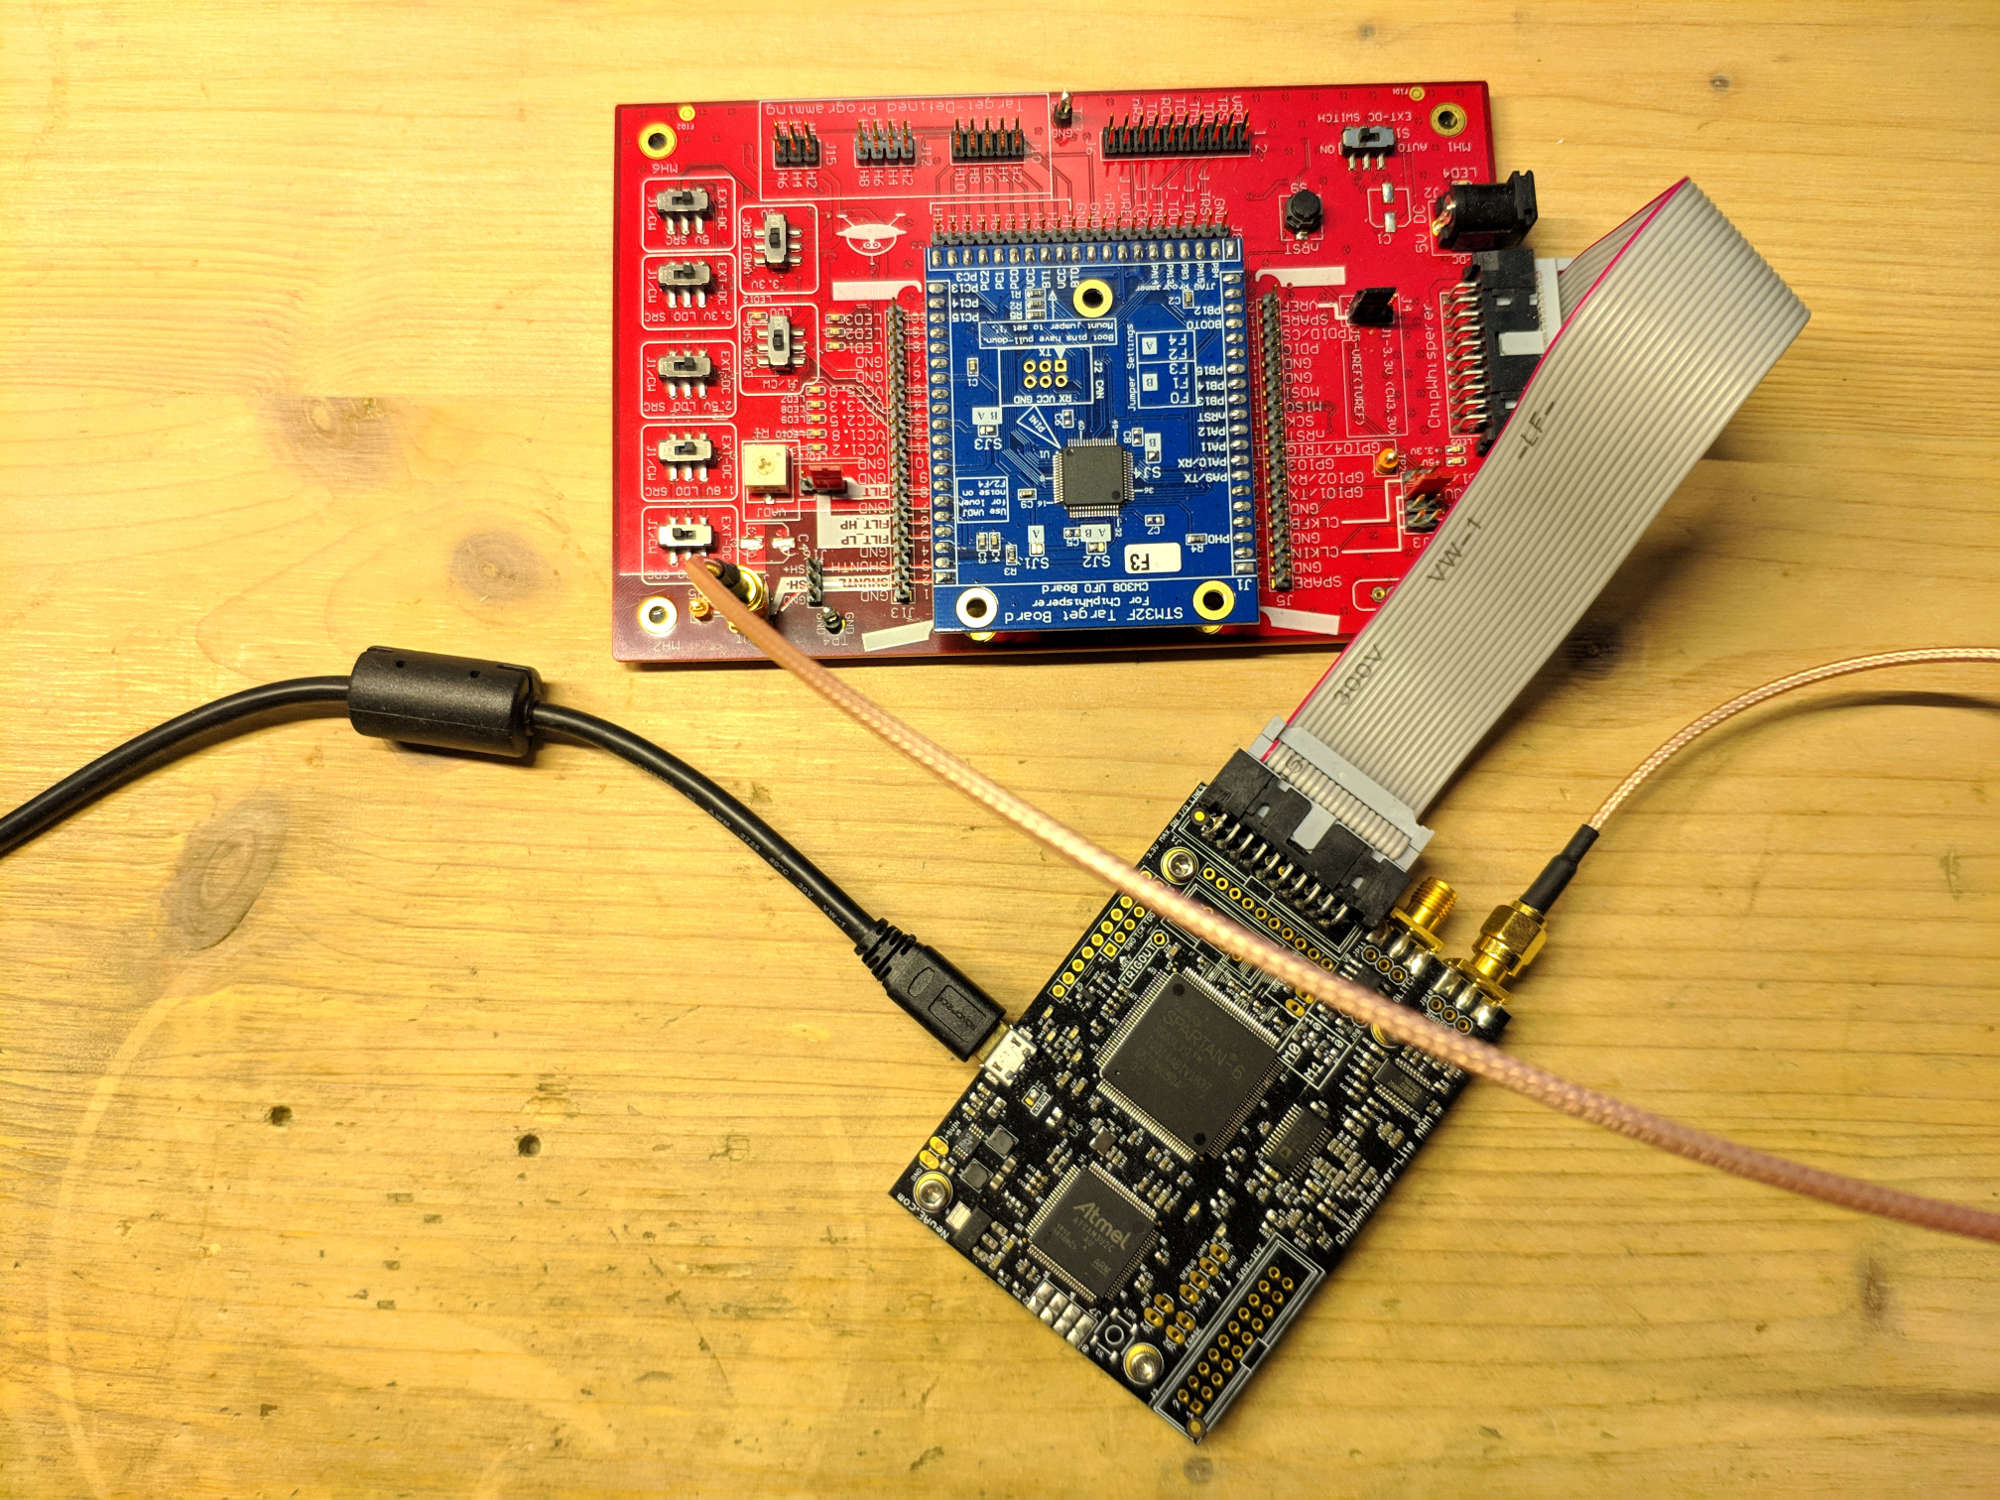
\includegraphics[width=\textwidth]{img/hw_setup.jpg}
\end{figure}

Das schwarze Board ist der ChipWhisperer, das rote Board ist das UFO-Board und
das blaue Board ist das Victim-Board. Der ChipWhisperer bietet Funktionalitäten
eines Oszilloskops, Programmers und kann z. B. präzise Clock- oder
Power-Glitches erzeugen. Für dieses Projekt relevant sind der Programmer und das
Aufzeichnen von Power-Traces. Dies geschieht über einen Shunt-Widerstand auf dem
Victim-Board. Die gemessene Spannung am Widerstand ist proportional zur
Stromaufnahme und wird nach einer Verstärkung auf dem ChipWhisperer über einen
zur Clock synchronisierten ADC abgetastet. Dadurch benötigt man eine im
Vergleich zum Oszilloskop wesentlich geringere Sample-Rate und produziert
dadurch auch weniger Daten.


\section{Software}

\subsection{Target}

Die Target-Software ist in C geschrieben und basiert auf dem Beispiel
\emph{simpleserial-aes}. Über die simpleserial-Schnittstelle, kann man sehr
einfach Befehle implementieren, die über eine eizige Zeile Code auf dem Host
ausgeführt werden können. Daher wurde auch in diesem Projekte die
simpleserial-Schnittstelle verwendet, um u. a. den zu verwendenden Schlüssel,
die Nonce oder den Klartext zu setzen - und vor allem, um den
Verschlüsselungsvorgang zu starten.


\subsection{Host}

Die Software basiert auf einer API des Herstellers NewAE, die als
Python-Bibliothek zur Verfügung gestellt wird. Damit ist es sehr einfach möglich
mit dem ChipWhisperer und dem Target zu kommunizieren. So kann man damit das
Target programmieren, Traces aufzeichnen und Analysen auf die Traces
durchführen. In diesem Projekt wird die Bibliothek jedoch nicht für Letzteres
benutzt. Hier bildet hauptsächlich die Bibliothek \emph{numpy} die Grundlage.


\subsection{Struktur}

\begin{itemize}
    \item doc: diese Dokumentation
    \item chacha: ChaCha-Implementierung sowie Known-Answer-Test
    \item target: Target-Implementierung
    \item attack: hauptsächlich Python-Skripte zur Durchführung des Angriffs
\end{itemize}




\chapter{Analyse}

\section{Erste Analyse und Vorgehensweise}

Wie in der Einführung erwähnt, ist ChaCha eine ARX-Chiffre. D. h. es werden
wiederholt die Operationen Addieren, Rotieren und exklusives Oder ausgeführt.
Diese Operationen benötigen zur Ausführung unabhängig von den Operanden immer
die gleiche Zeit. Damit ist ein Timing-Angriff ausgeschlossen.

Eine Möglichkeit ChaCha über einen Seitenkanal anzugreifen, ist die Correlation
Power Analysis. Diese Variante wird in diesem Projekt untersucht und
vorgestellt. Vor dem Angriff wird eine Analyse des Leakages durchgeführt.
Leakage ist das ungewollte Verlassen von Informationen aus dem Gerät. Dies kann
man mit dem spezifischen TVLA (Test Vector Leakage Assessment) oder NICV
(Normalized Inter Class Variance) feststellen.

Der hier durchgeführte Angriff orientiert sich am Paper
\cite{jungk_bhasin_2017}. Es werden zwei Varianten vorgestellt. Bei der ersten
Variante hat der Angreifer volle Kontrolle über alle Eingabedaten, also den
Counter und die Nonce. In der zweiten Variante hat der Angreifer nur Kontrolle
über die beiden letzten Wörter der Nonce. Der Counter sowie das erste Wort der
Nonce haben einen konstanten und bekannten Wert. In der ersten Variante können
alle acht 32-bit Subkeys (Teile des Schlüssels) direkt in der ersten Runde
angegriffen werden. In der zweiten Variante können vier der acht 32-bit Subkeys
in der ersten Runde angegriffen werden. Die restlichen vier Subkeys werden
indirekt angegriffen, indem der Zustand der entsprechenden Subkeys nach der
ersten Runde angegriffen wird. Dann kann man den vorherigen Zustand mit der
inversen Rundenfunktion berechnen, welcher die gesuchten restlichen Subkeys
beinhaltet. Beide Varianten werden in diesem Projekt untersucht.


\section{Target vorbereiten}

Bevor die Traces aufgezeichnet werden können, muss das Target wie in
\autoref{sec:hw-setup} beschrieben aufgebaut werden. Anschließend muss das
Target programmiert werden. Dies ist im \autoref{lst:program-target}
beschrieben.

\begin{lstlisting}[language=bash, caption={Target programmieren}, label=lst:program-target]
./build_target.sh
./program_target.py
\end{lstlisting}


\section{Aufzeichnen von Traces}

Für die Analyse und den Angriff werden mehrere Aufzeichnungen durchgeführt,
wobei jede Aufzeichnung einige Hundert Traces beinhaltet. Jede Aufzeichnung hat
einen festen zufälligen Schlüssel. Der Counter und die Nonce haben je nach
Parametern entweder einen festen Wert oder werden für jeden Trace zufällig neu
generiert. Damit können Traces für beide im vorherigen Abschnitt vorgestellten
Varianten des Angriffs aufgezeichnet werden. Die genannten Parameter werden
zusammen mit den Traces gespeichert. Der Klar- sowie Schlüsseltext werden nicht
gespeichert, da diese für den hier durchgeführten Angriff nicht relevant sind
und daher die Aufzeichnung der Traces unnötig verlangsamen würden, weil dann
eine erheblich größere Datenmenge zum und vom Target übertragen werden muss.

Für die erste Analyse mit TVLA und NICV reicht bereits eine Aufzeichnung einer
Menge von Traces aus. Zur Analyse des Angriffs werden mindestens zehn
Aufzeichnungen benötigt. Bei der ersten Variante sind Counter und Nonce frei
wählbar, weshalb diese für jeden Trace neu zufällig generiert werden. Bei der
zweiten Variante sind nur die letzten beiden Wörter der Nonce frei wählbar,
weshalb diese für jeden Trace neu zufällig generiert werden. Der Counter und das
erste Wort der Nonce werden auf einen festen zufälligen Wert gesetzt.

Das Aufzeichnen der Traces wird mit dem Skript \emph{capture\_traces.py}
durchgeführt. Zunächst werden 100 Aufzeichnungen mit je 500 Traces durchgeführt.
Dieser Schritt ist in beiden Listings \autoref{lst:capture-1} und
\autoref{lst:capture-2} (bis auf die Option \verb+-r+) gleich. Anschließend
werden bei der zweiten Variante zu den Aufzeichnungen weitere Aufzeichnungen mit
dem gleichen Eingabedaten erstellt, bei denen jedoch das zweite Wort der Nonce
auf \emph{0x55555555} fixiert wird. Dies hat den Hintergrund, dass sich bei
Berechnungen mit diesen Eingabedaten (zweites Wort der Nonce) möglichst viele
Bits ändern und dadurch die Wahrscheinlichkeit gesenkt wird, dass man zufällig
passende Korrelationen mit falschen Daten erhält (mehr dazu später). Warum diese
Aufzeichnungen überhaupt benötigt werden, wird im entsprechenden Abschnitt beim
Angriff erklärt. Bei der Analyse werden sie noch nicht benötigt.

\begin{lstlisting}[language=bash, caption={Traces für Variante 1 aufzeichnen}, label=lst:capture-1]
./capture_traces.py -s 100 -t 500
\end{lstlisting}

\begin{lstlisting}[language=bash, caption={Traces für Variante 2 aufzeichnen}, label=lst:capture-2]
./capture_traces.py -s 100 -t 500 -r
./capture_traces.py -s 100 -t 500 -r -1 traces_*.npz
\end{lstlisting}


\section{Spezifisches TVLA \& NICV}

TVLA und NICV sind zwei unterschiedliche Methoden, um auf eine einfache Art und
Weise Leakage festzustellen. In diesem Projekt wird es benutzt, um zu
Überprüfen, ob der Aufbau korrekt ist und um die relevanten Samples für den
Angriff auszuwählen, wodurch dieser erst möglich wird.

Bei beiden Methoden werden die Traces abhängig von den Werten bestimmter
Zwischenzustände (``intermediates'') in mehrere Gruppen unterteilt. Anschließend
werden diese mit Hilfe statistischer Funktionen ausgewertet. Beim TVLA wird der
Welch's t-Test angewendet, beim NICV wird das Leakage über die Varianzen der
Gruppen berechnet. Für beide Methoden gibt es ein entsprechendes Skript, welches
einen Graph der entsprechenden Werte erzeugt. Beispiele sind in
\autoref{lst:leakage-plot} zu sehen.

\begin{lstlisting}[language=bash, caption={Plots von TVLA \& NICV}, label=lst:leakage-plot]
./tvla_specific.py traces_0.npz
./nicv.py traces_0.npz
./plot_trace.py traces_0.npz
\end{lstlisting}

\medskip

Die erzeugten Plots der in \autoref{lst:leakage-plot} gezeigten Skripte sind in
den Abbildungen \autoref{fig:plot-tvla} für TVLA bzw. \autoref{fig:plot-nicv}
für NICV zu sehen. Zur Einordnung ist in \autoref{fig:plot-power-trace} der
Power-Trace zu sehen. Dort erkennt man, dass ca. ab dem Sample 1500 die erste
Doppel-Runde beginnt, welche ca. beim Sample 3400 endet. In
\autoref{fig:plot-tvla-bytes} ist die TVLA-Analyse pro Byte anstatt pro 32-bit
Subkey zu sehen, welche die Grundlage für die anschließende Auswahl der
relevanten Samples bildet.

\begin{figure}[H]
    \caption{TVLA: Übersicht}
    \label{fig:plot-tvla}

    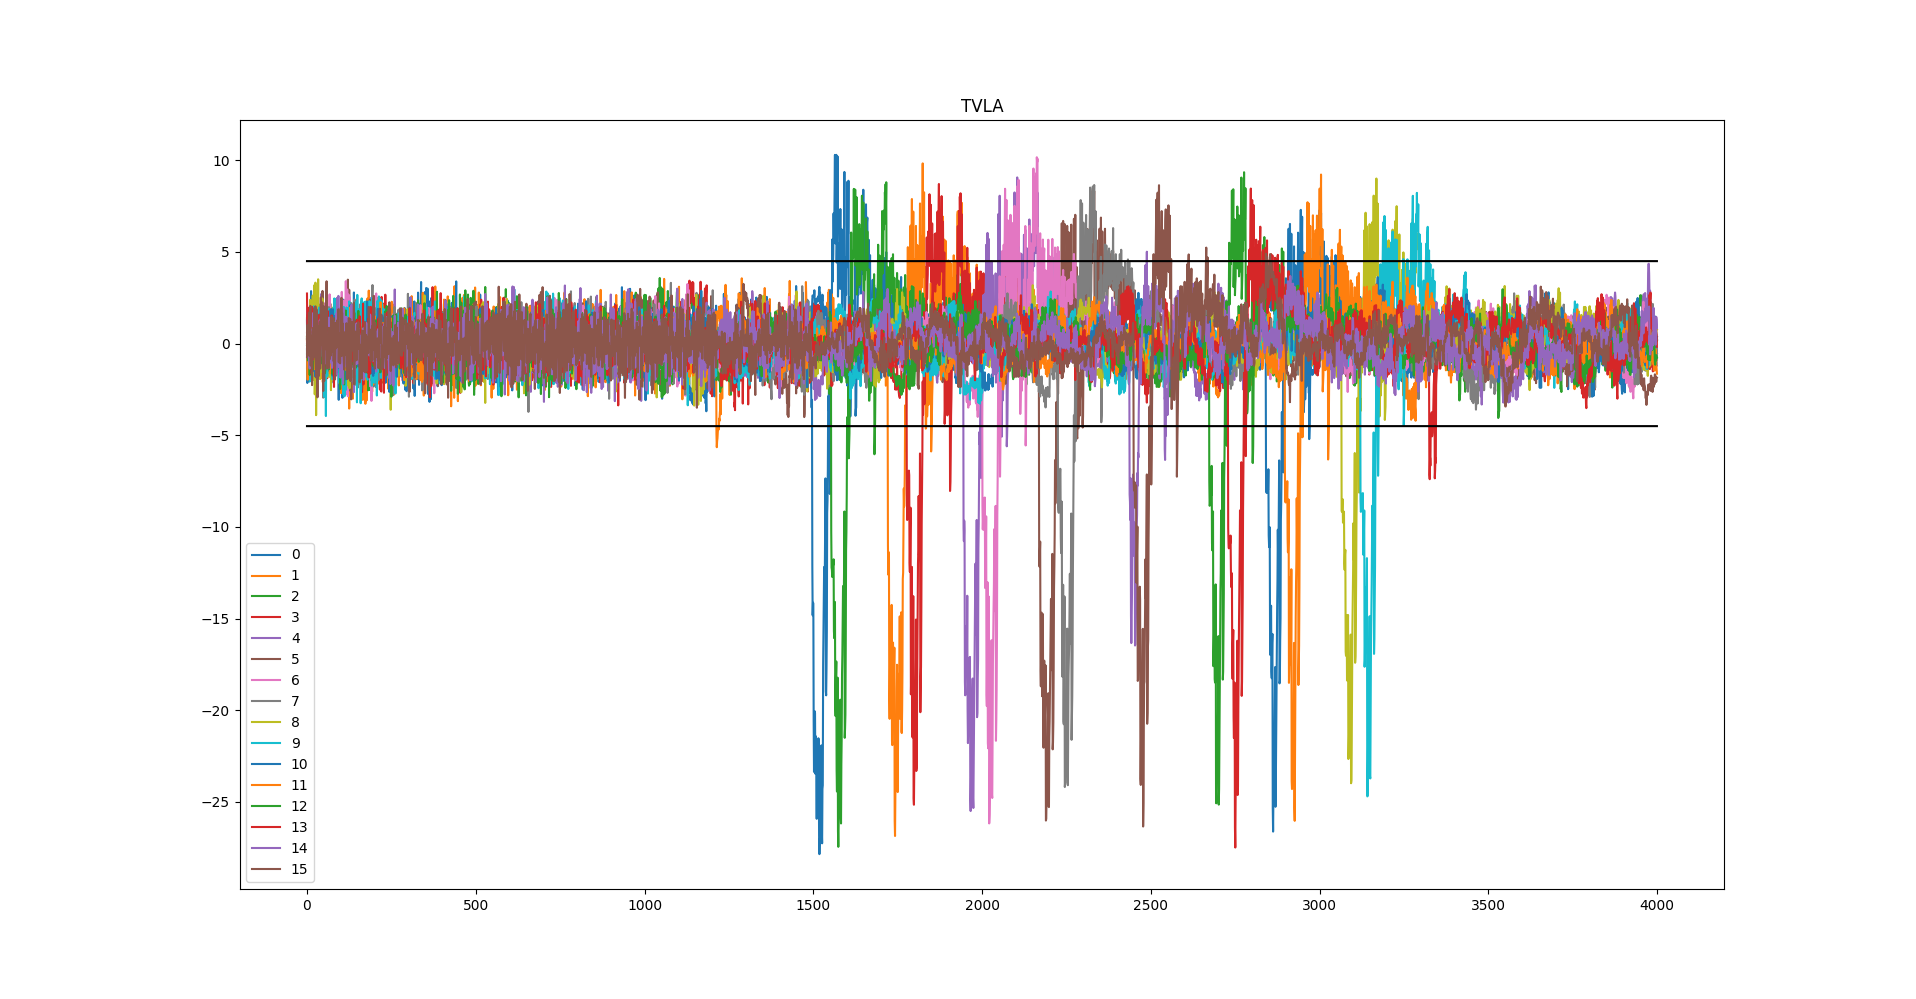
\includegraphics[width=\textwidth]{img/tvla_specific_overview.png}
\end{figure}

\begin{figure}[H]
    \caption{NICV: Übersicht}
    \label{fig:plot-nicv}

    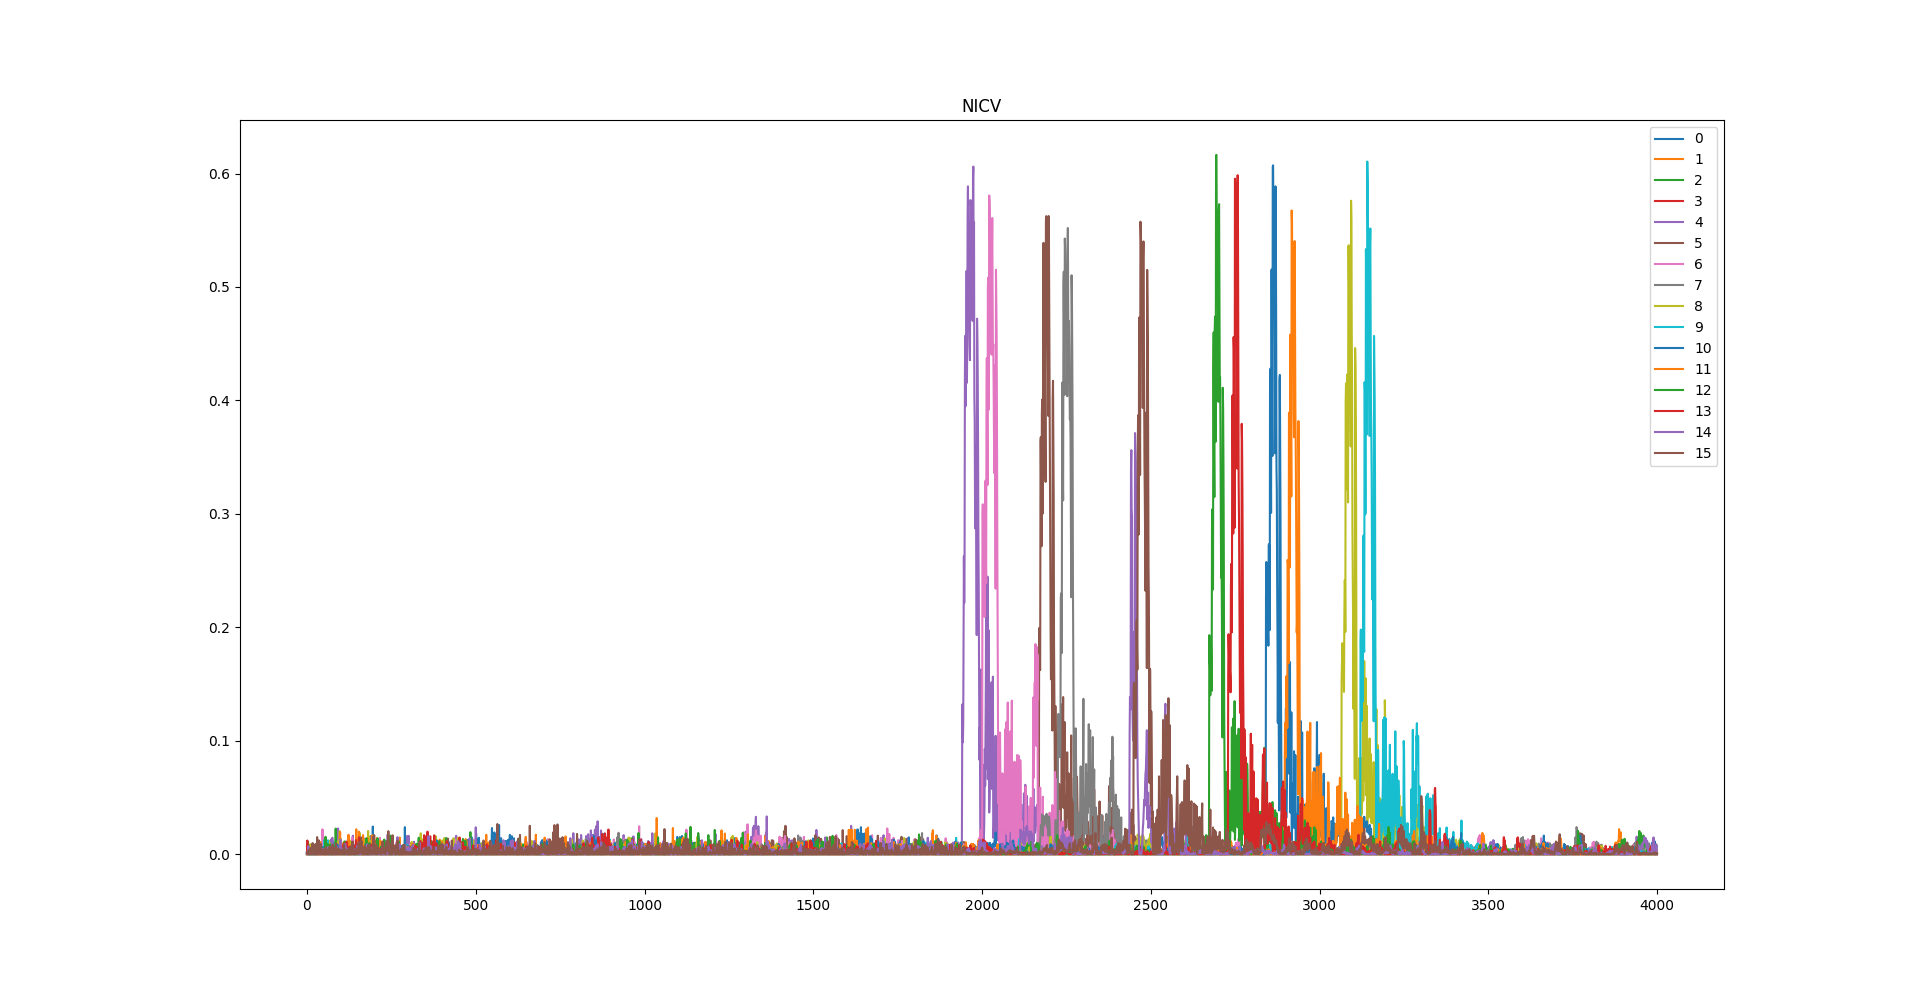
\includegraphics[width=\textwidth]{img/nicv_overview.png}
\end{figure}

\begin{figure}[H]
    \caption{Power-Trace}
    \label{fig:plot-power-trace}

    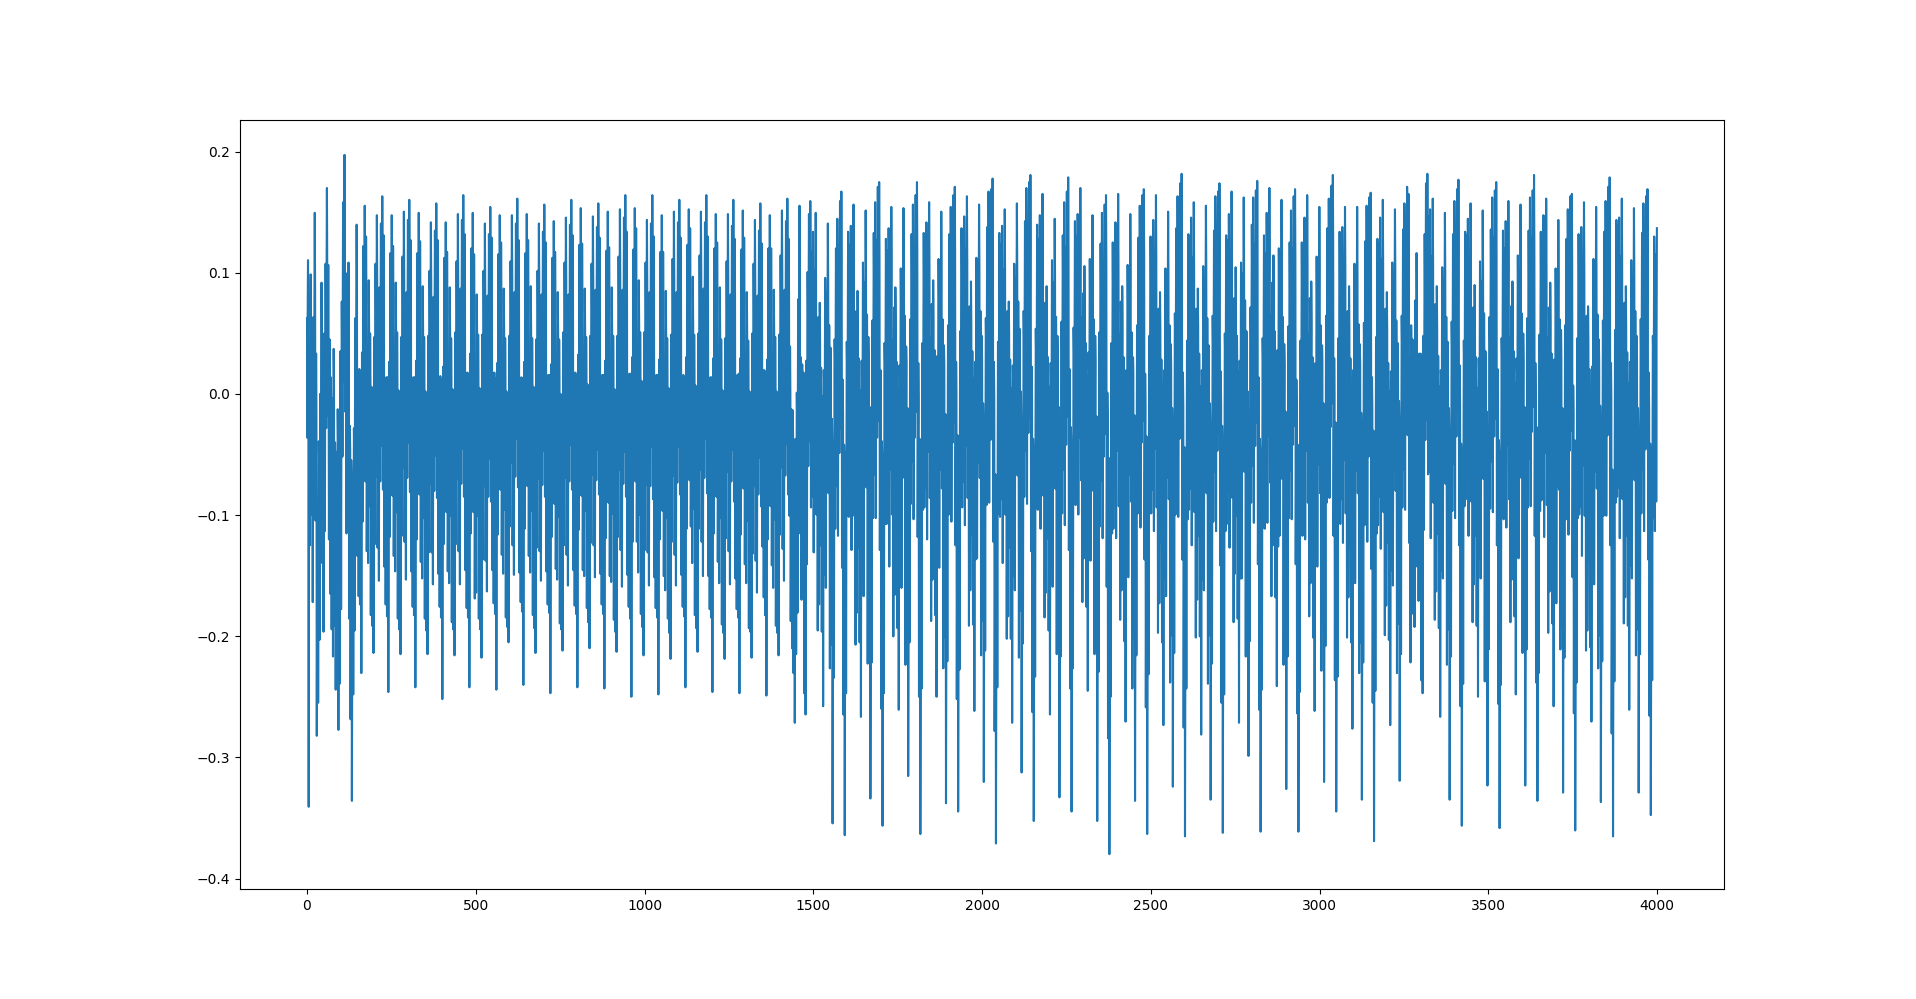
\includegraphics[width=\textwidth]{img/power_trace.png}
\end{figure}

\begin{figure}[H]
    \caption{TVLA: Bytes}
    \label{fig:plot-tvla-bytes}

    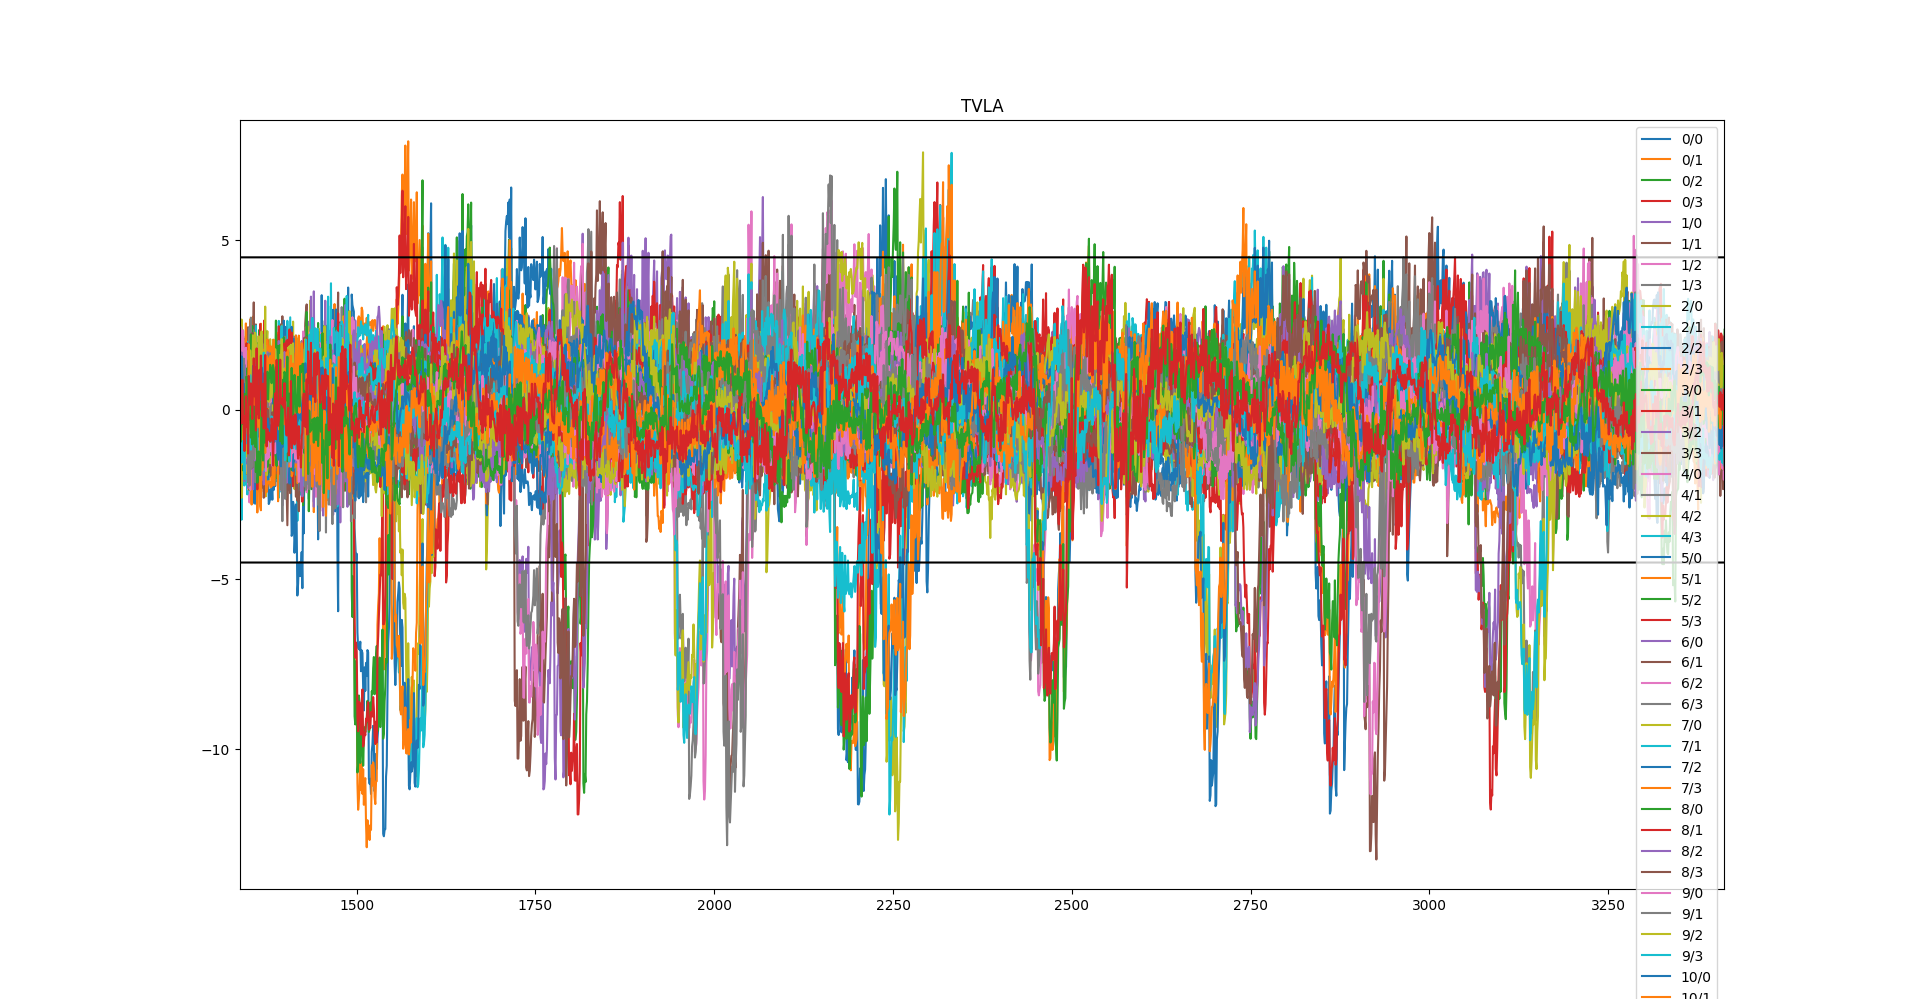
\includegraphics[width=\textwidth]{img/tvla_specific_bytes.png}
\end{figure}


\section{Relevante Samples auswählen}
\label{sec:select-relevant-samples}

Das Auswählen der relevanten Samples geschieht hier nur mit TVLA und ist
unabhängig von der durchgeführten Variante. Ein Beispiel ist in
\autoref{lst:select-samples} dargestellt. Eine Auswahl auf Basis von NICV wäre
wahrscheinlich auch möglich, wird aber im Rahmen dieses Projekts nicht
untersucht.

\begin{lstlisting}[language=bash, caption={Samples auswählen}, label=lst:select-samples]
./tvla_calc_subkey_samples.py traces_[0-9].npz
\end{lstlisting}

\medskip

Hierbei wird jede Aufzeichnung mit TVLA analysiert und für jedes Byte des
Schlüssels ein Score berechnet. Jeweils das Sample mit dem höchsten absoluten
TVLA-Wert bekommt 21 Punkte. Das Sample mit dem zweithöchsten Wert bekommt 20
Punkte, usw.  Am Ende werden die fünf Samples mit dem höchsten Score ausgewählt
und in der Datei \emph{subkey\_samples.py} gespeichert. Da diese Datei eine
Textdatei ist, kann diese nacher angesehen und bearbeitet werden.

Für brauchbare Werte sollte man bei 500 Traces pro Aufzeichnung mindestens zehn
Aufzeichnungen (wie im \autoref{lst:select-samples} gezeigt) angeben, da das
Leakage einem gewissen Rauschen unterliegt, welches durch mehrere Aufzeichnungen
kompensiert werden soll.


\section{ChaCha Algorithmus}

Um den Angriff im folgenden Kapitel zu verstehen, ist es notwendig zu wissen,
wie der Algorithmus, der den Schlüsselstrom berechnet, funktioniert.

ChaCha arbeitet mit einem internen Zustand. Dieser wird anfangs wie in
\autoref{lst:chacha-init} gezeigt initialisiert. Alle Teile des Zustands v0-v15
liegen im little-endian Format vor.

\begin{lstlisting}[caption={Initialer Zustand}, label=lst:chacha-init]
v0  = C0        v1  = C1        v2  = C2        v3  = C3
v4  = k0        v5  = k1        v6  = k2        v7  = k3
v8  = k4        v9  = k5        v10 = k6        v11 = k7
v12 = counter   v13 = nonce0    v14 = nonce1    v15 = nonce2

C0 = 0x61707865         # 'expa'
C1 = 0x3320646e         # 'nd 3'
C2 = 0x79622d32         # '2-by'
C3 = 0x6b206574         # 'te k'
\end{lstlisting}

\medskip

Anschließend werden 20 Runden auf diesem Zustand ausgeführt. Am Ende wird der
initiale Zustand hinzuaddiert. Nach dem Serialisieren der Daten, also dem
Umwandeln der 32-bit Integer in Bytes, erhält man den Schlüsselstrom. In den 20
Runden wird jeweils vier Mal die \emph{quarterround} ausgeführt. Dies geschieht
abwechselnd je mit allen Spalten vertikal (z. B. v0, v4, v8, v12) und quer von
links oben nach rechts unten (z. B. v0, v5, v10, v15). Dies ist in
\autoref{lst:chacha-double-round} dargestellt.

\begin{lstlisting}[caption={ChaCha Doppel-Runde}, label=lst:chacha-double-round]
v0',  v4',  v8',  v12' = quarterround(v0,  v4,  v8,  v12)
v1',  v5',  v9',  v13' = quarterround(v1,  v5,  v9,  v13)
v2',  v6',  v10', v14' = quarterround(v2,  v6,  v10, v14)
v3',  v7',  v11', v15' = quarterround(v3,  v7,  v11, v15)

v0'',  v5'',  v10'', v15'' = quarterround(v0',  v5',  v10', v15')
v1'',  v6'',  v11'', v12'' = quarterround(v1',  v6',  v11', v12')
v2'',  v7'',  v8'',  v13'' = quarterround(v2',  v7',  v8',  v13')
v3'',  v4'',  v9'',  v14'' = quarterround(v3',  v4',  v9',  v14')
\end{lstlisting}

\medskip

In der \emph{quarterround} werden die Rechenoperationen auf den Daten
ausgeführt. Diese sind in Listing \autoref{lst:chacha-quarterround} dargstellt.

\begin{lstlisting}[caption={ChaCha quarterround}, label=lst:chacha-quarterround]
Alle Variablen sind 32-bit Woerter!
x << n := rotate_left(x, n)

Parameter: a0, b0, c0, d0

a1 = a0 + b0    d1 = d0 ^ a1    d2 = d1 << 16
c1 = c0 + d2    b1 = b0 ^ c1    b2 = b1 << 12
a2 = a1 + b2    d3 = d2 ^ a2    d4 = d3 << 8
c2 = c1 + d2    b3 = b2 ^ c2    b4 = b3 << 7

return a2, b4, c2, d4
\end{lstlisting}




\chapter{Angriff}

\section{Einführung}

In diesem Projekt wird ChaCha mit Hilfe der Correlation Power Analysis
angegriffen. Jedes 32-bit Wort des Schlüssels wird im Code \emph{externer
Subkey} genannt. Jedes Byte eines externen Subkeys wird im Code \emph{interner
Subkey} genannt. Außerdem wird im Folgenden zwischen den beiden Varianten
(Angreifer hat die volle oder eingeschränkte Kontrolle über die Parameter)
unterschieden, da sich die Angriffe hier teils stark unterscheiden.


\section{Correlation Power Analysis}
\label{sec:cpa}

CPA ist eine Methode, um Power-Traces zu analysieren. Dafür zeichnet man
zunächst einige Hundert Power-Traces auf. Dann stellt man ein Modell für den
Stromverbrauch einer bestimmten Operation abhängig von den Operanden auf. Man
kann sich darunter eine Vorhersage des Stromverbrauchs vorstellen. Anschließend
berechnet man die Korrelation für jedes Sample der Traces mit dem Modell. Eine
hohe Korrelation spricht dafür, dass das Modell zum beobachteten Stromverbrauch
passt und damit die verwendeten Argumente wahrscheinlich die sind, die die CPU
bei der Operation verwendet hat.

Das Modell berechnet den Stromverbrauch basierend auf einem Zwischenwert
(``intermediate''), der sich aus bekannten und unbekannten Daten zusammensetzt.
Ziel ist es, die unbekannten Daten zu ermitteln. Dazu stellt man für alle
möglichen (unbekannten) Eingabedaten ein Modell auf und berechnet die
Korrelation. Das Modell, das am besten mit den Traces korreliert, ist vermutlich
die korrekte ``Vorhersage'' und hat die richtigen Eingabedaten. Allgemein lässt
sich ein Modell wie in \autoref{lst:cpa-model} zu sehen beschreiben.

\begin{lstlisting}[caption={Allgemeines Modell für Stromverbrauch}, label=lst:cpa-model]
float x = model(intermediate(known_data, unknwon_data))
\end{lstlisting}

\medskip

Die Berechnung der Korrelation wird für jedes Sample (das zuvor im
\autoref{sec:select-relevant-samples} ausgewählt wurde) durchgeführt.
Anschließend wird üblicherweise für jedes Modell die maximale absolute
Korrelation als beste Korrelation genommen. In diesem Projekt hat sich hierbei
jedoch ein anderer Ansatz als besser herausgestellt: Dabei berechnet man
zunächst wieder die Korrelation aller Modelle für jedes Sample. Anschließend
bestimmt man für jedes Sample das Modell mit der höchsten absoluten Korrelation.
Dann zählt man für jedes Modell, wie oft es am besten war. Das Modell, das am
öftesten ``gewonnen'' hat, hat am wahrscheinlichsten die korrekten Eingabedaten.


\section{Modelle für CPA}

Um den Stromverbrauch zu modellieren gibt es mehrere Varianten von denen man
eine zum Target und zur Implementierung passend wählen muss. Die zwei gängigsten
Modelle sind das \emph{Hamming-Weight}- und \emph{Hamming-Distance}-Modell. Das
HW-Modell gibt die Anzahl der 1-Bits eines Worts an. Das HD-Modell gibt die
Anzahl der Bits an, die sich ändern, wenn man ein Wort durch ein anderes
ersetzt. Damit entspricht \verb+HD(a, b) = HW(a ^ b)+.

Die Operationen, die die CPU ausführt, leaken auf unterschiedliche, aber
bestimmte Arten Informationen. Oft funktioniert jedoch das HW-Modell sehr gut,
vor allem dann, wenn man Zwischenwerte angreifen möchten, die vom RAM geladen
oder ins RAM geschrieben werden. Die Angriffe in diesem Projekt basieren alle
auf dem HW-Modell.


\section{Variante 1}

Bei der ersten Variante hat der Angreifer die volle Kontrolle über alle
Eingabedaten. D. h er kann den Counter und die Nonce steuern. Daher werden beim
Aufzeichnen der Traces der Counter und die Nonce für jeden Trace zufällig neu
gewählt. So kann man jetzt zunächst die erste Hälfte des Schlüssels (k0-k3)
angreifen. Dazu verwendet man das in \autoref{lst:cpa-model-0} beschriebene
Modell.

\begin{lstlisting}[caption={Modell für Stromverbrauch}, label=lst:cpa-model-0]
HW(d1) = HW(d0 ^ a1) = HW(d0 ^ (a0 + b0))
\end{lstlisting}

\medskip

Die Subkeys k0-k3 liegen im Zustand in v4-v7. Damit werden diese an
\emph{quarterround} als Parameter b übergeben. Der Parameter a ist entsprechend
v0-v3, d ist entsprechend v12-v15. v0-v3 sind die Konstanten C0-C3, v12-v15 sind
die frei wählbaren und bekannten Eingabedaten (Counter und Nonce). Die neuen
Modelle mit den bekannten Parametern sind in \autoref{lst:cpa-model-1}
dargestellt.

\begin{lstlisting}[caption={Modell für Stromverbrauch von d1}, label=lst:cpa-model-1]
k0: HW(d1) = HW(counter ^ (C0 + k0))
k1: HW(d1) = HW(nonce0  ^ (C1 + k1))
k2: HW(d1) = HW(nonce1  ^ (C2 + k2))
k3: HW(d1) = HW(nonce2  ^ (C3 + k3))
\end{lstlisting}

\medskip

Aufgrund des XORs erhält man eine punktsymmetrische Verteilung der maximalen
Korrelationen der Subkeys. D. h. es gibt mindestens zwei Modelle, die die
gleiche absolute Korrelation haben, wobei eine der Korrelationen positiv und die
andere Korrelation negativ ist. In diesem Projekt hat sich herausgestellt, dass
nie das Modell mit der positiven Korrelation korrekt ist, weshalb man hier alle
positiven Korrelationen ignoriert und nach der kleinsten Korrelation sucht.
\autoref{fig:xor-symmetry} zeigt beispielhaft die vier besten absoluten
Korrelationen und damit die Symmetrie.

\begin{figure}[H]
    \caption{Symmetrische Verteilung}
    \label{fig:xor-symmetry}

    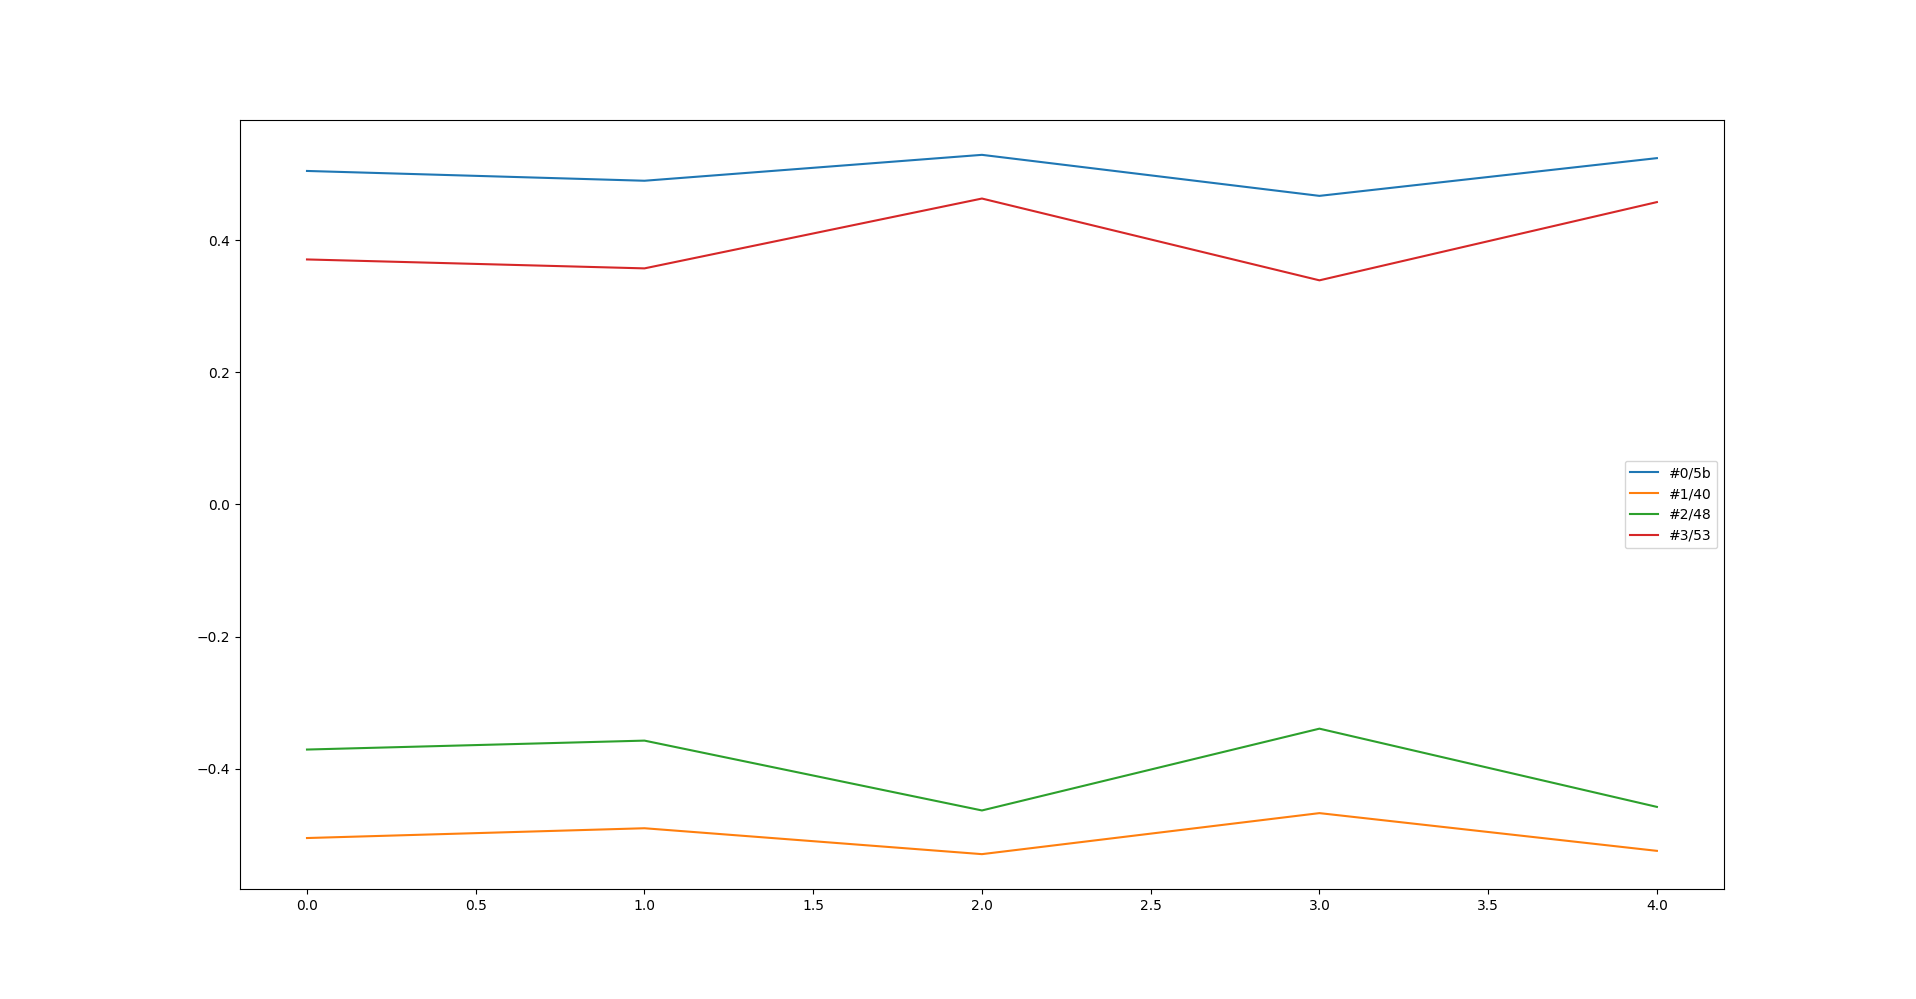
\includegraphics[width=\textwidth]{img/corrs_subkey_byte.png}
\end{figure}


Da k0-k3 32-bit Wörter sind, wäre ein Angriff auf das jeweilige ganze Wort zu
aufwendig. Daher wird hier mit dem Prinzip \emph{divide and conquer} (dt.
``teile und herrsche'') vorgegangen. Aufgrund der Addition wird zunächst das LSB
angegriffen. Danach werden die nächsten Bytes angegriffen, wobei die vorherigen
Bytes mitverwendet werden müssen, da ansonsten der Übertrag bei der Addition
möglicherweise nicht stimmt und dadurch das Ergebnis um 1 neben dem richtigen
Ergebnis liegt.

Nachdem k0-k3 bestimmt wurden, ist es möglich k4-k7 anzugreifen. Dazu verwendet
man das in \autoref{lst:cpa-model-2} gezeigte Modell.

\begin{lstlisting}[caption={Modell für Stromverbrauch von b1}, label=lst:cpa-model-2]
HW(b1) = HW(b0 ^ c1) = HW(b0 ^ (c0 + d2)) = HW(b0 ^ (c0 + (d1<<16)))
       = HW(b0 ^ (c0 + ((d0 ^ a1)<<16)))
       = HW(b0 ^ (c0 + ((d0 ^ (a0 + b0))<<16)))

k4: HW(b1) = HW(k0 ^ (k4 + ((counter ^ (C0 + k0))<<16)))
\end{lstlisting}

\medskip

Hier setzt man für a, b und d wieder die gleichen Werte ein. Zusätzlich muss man
hier noch für c die Werte k4-k7 einsetzen. Damit ist hier a, b und d bekannt und
c der gesuchte Werte. Ein Beispiel für k4 ist in \autoref{lst:cpa-model-2}
gegeben.

Auch hier wird wieder mit dem \emph{divide-and-conquer}-Prinzip vorgegangen. Im
Gegensatz zum vorherigen Modell für die erste Hälfte des Schlüssels, ist das
Ergebnis hier nicht symmetrisch, weshalb die höchste absolute statt der
kleinsten Korrelation als die beste Korrelation gewertet wird.

Der Angriff ist damit abgeschlossen, alle Teile des Schlüssels wurden
angegriffen. Die Durchführung des Angriffs ist im \autoref{lst:attack-1}
gezeigt.

\begin{lstlisting}[language=bash, caption={Angriff, Variante 1}, label=lst:attack-1]
./attack.py traces_0.npz
\end{lstlisting}


\section{Variante 2}
\label{sec:attack-2}

Bei der zweiten Variante kann der Angreifer nur das zweite und dritte Wort der
Nonce bzw. v14 und v15 steuern. Der Counter und das erste Wort der Nonce sind
nicht beeinflussbar, aber konstant und bekannt. Damit ist der Angreifer in der
Lage, genau wie bei der ersten Variante die Subkeys k2, k3, k6 und k7 zu
berechnen. Anschließend kann man die Wörter v4', v9', v13', v8', v12', v1', v0'
und v5' in genannter Reihenfolge angreifen. Dazu werden die Wörter v2', v3',
v6', v7', v10', v11', v14' und v15' benötigt, welche mit der
\emph{quarterround}-Funktion aus den bereits bekannten Subkeys k2, k3, k6 und k7
berechnet werden können. Die restlichen Parameter sind Konstanten oder das
zweite bzw. dritte Wort der Nonce. Der weitere Angriff läuft dann wie folgt ab:

\begin{enumerate}
    \item v4' soll berechnet werden. Dafür werden die Modelle in den Zeilen 1-2
        des \autoref{lst:cpa-model-3} verwendet. Im Listing ist jeweils als
        erstes das zu berechnende Wort angegeben. Dann folgt ein Pfeil, hinter
        dem die dazu entsprechende Variable (die ermittelt werden soll) steht.
        Darauf folgt dann das eigentliche Modell, zunächst allgemein und dann
        mit den eingesetzten Variablen. In der jeweils letzten Zeile sieht man,
        dass bis auf die gesuchte Variable alle anderen Variablen bekannt sind.
        Das Ergebnis hier ist nicht symmetrisch, weshalb die beste absolute
        Korrelation gewählt wird. Sofern in den weiteren Schritten nicht anders
        angegeben, ist davon auszugehen, dass das Ergebnis nicht symmetrisch
        ist.

    \item v9', v13' und v8' sollen berechnet werden. Man verfährt analog zur
        Berechnung von v4', wobei das Ergebnis von v13' symmetrisch ist, weshalb
        die beste negative Korrelation gewählt wird.

    \item v12' soll berechnet werden. v12' kann nicht direkt berechnet werden,
        stattdessen wird d2 der entsprechenden \emph{quarterround} berechnet.
        Ansonsten läuft der Angriff analog zu den vorherigen Berechnungen, wobei
        beachtet werden muss, dass d2 konstant sein muss. In den vorherigen
        Schritten war dies immer gegeben, hier muss man prüfen, von welchen
        Variablen d2 abhängt. In diesem Fall sind das a0, b0 und d0. Diese
        Variablen entsprechen v1', v6' und v12'. v1' und v12' stehen in den
        beiden linken Spalten. Damit wären diese abhängig vom Counter und dem
        ersten Wort der Nonce. Diese beiden Wörter werden aber als konstant
        vorausgesetzt, weshalb v1' und v12' konstant sind. v6' ist abhängig vom
        zweiten Wort der Nonce. Damit v6' konstant ist, muss also das zweite
        Wort der Nonce konstant sein. Aus diesem Grund wurden beim Aufzeichnen
        der Traces weitere Aufzeichnungen mit dem zweiten Wort der Nonce
        konstant erstellt. Diese Aufzeichnung müssen nun hier verwendet werden.

    \item v1' soll berechnet werden. Auch hier wird v1' nicht direkt berechnet,
        sondern a1. Außerdem werden die Variablen nicht bis zum Ursprung (also
        a0, b0, c0, d0) ersetzt, sodass man für d2 den im vorherigen Schritt
        berechneten Wert einsetzen kann. Anders würde es auch nicht
        funktionieren, da man dann a0, b0 und d0 kennen müsste, was v1', v6' und
        v12' entspricht. v6' ist bekannt, v1' und v12' jedoch nicht. Bezüglich
        der Aufzeichnungen gilt hier das gleiche wie im vorherigen Schritt, da
        auch hier d2 verwendet wird und daher konstant sein muss. Damit a1
        konstant ist muss a0 und b0 konstant sein, was bereits im vorherigen
        Schritt gezeigt wurde.
    \label{itm:calc-v1}

    \item v12' und v1' berechnen. Aus den Zwischenwerten d2 sowie a1 kann nun d0
        sowie a0 berechnet werden. Damit erhält man v12' bzw v1'.

    \item v0' soll berechnet werden. Auch hier kann v0' nicht direkt berechnet
        werden. Stattdessen wird mit einem kleinen Unterschied analog zu den
        vorherigen Schritten a1 berechnet. Hier muss das Ergebnis der
        intermediate-Funktion um 16 Bits nach rechts rotiert werden. Dies liegt
        daran, dass die Variable, die berechnet werden soll durch das
        \emph{rotate left} beeinflusst wird. Diese Verschiebung muss man am Ende
        wieder rückgängig machen. Das Ergebnis wird dadurch nicht verfälscht, da
        die \emph{rotate}-Operation das Hamming-Gewicht der gesamten Variable
        nicht ändert. Bei diesem Schritt werden wieder die ``normalen''
        Aufzeichnungen mit zufälligem zweiten Wort der Nonce verwendet, da hier
        a1 von a0 und b0, also von v0' und v5' abhängig ist. Diese beiden Werte
        stehen in den beiden linken Spalten und sind daher wie in den Schritten
        zuvor erklärt konstant.

    \item v5' soll berechnet werden. Dies geht direkt, jedoch darf man auch hier
        die Variablen nicht bis zum Schluss auflösen, sodass man a1 aus dem
        vorherigen Schritt einsetzen kann. Außerdem ist das Ergebnis hier
        symmetrisch, weshalb die beste negative Korrelation gewählt wird.

    \item v0' berechnen. v0' kann aus a1, was zuvor ermittelt wurde und dem
        bekannten Wert v5' aus dem vorherigen Schritt berechnet werden.
\end{enumerate}


\begin{lstlisting}[caption={Modelle für Stromverbrauch}, label=lst:cpa-model-3]
v4'  -> b0: HW(d1) = HW(d0 ^ (a0 + b0))
                   = HW(v14' ^ (v3' + v4'))
v9'  -> c0: HW(b1) = HW(b0 ^ (c0 + ((d0 ^ (a0 + b0))<<16)))
                   = HW(v4' ^ (v9' + ((v14' ^ (v3' + v4'))<<16)))

v13' -> d0: HW(d1) = HW(d0 ^ (a0 + b0))
                   = HW(v13' ^ (v2' + v7'))
v8'  -> c0: HW(b1) = HW(b0 ^ (c0 + ((d0 ^ (a0 + b0))<<16)))
                   = HW(v7' ^ (v8' + ((v13' ^ (v2' + v7'))<<16)))

v12' -> d2: HW(b1) = HW(b0 ^ (c0 + d2))
                   = HW(v6' ^ (v11' + d2))
v1'  -> a1: HW(d3) = HW(d2 ^ ((a0 + b0) + ((b0 ^ (c0 + d2))<<12)))
                   = HW(d2 ^ ((v1' + v6') + ((v6' ^ (v11' + d2))<<12)))

v1':  a0 = a1 - b0
         = a1 - v6'
v12': d0 = (d2>>16) ^ a1

v0'  -> a1: HW(c1>>16) = HW((c0 + ((d0 ^ a1)<<16))>>16)
                       = HW((v10' + ((v15' ^ a1)<<16))>>16)
v5'  -> b0: HW(b1) = HW(b0 ^ (c0 + ((d0 ^ a1)<<16)))
                   = HW(v5' ^ (v10' + ((v15' ^ a1)<<16)))

v0':  a0 = a1 - b0
         = a1 - v5'
\end{lstlisting}

\medskip

Nachdem alle Schritte ausgeführt wurden, sind die Wörter der ersten beiden
Spalten nach der ersten Runde bekannt (v0', v1', v4', v5', v8', v9', v12',
v13'). Nun kann man die Werte aus der ersten Runde mit der inversen
\emph{quarterround} berechnen. Damit erhält man die restlichen Subkeys k0, k1,
k4 und k5. Außerdem kann man nun überprüfen, ob v0, v1, v12 und v13 die
richtigen Werte beinhalten. v0 müsste gleich C0, v1 gleich C1, v12 gleich dem
Counter und v13 gleich dem ersten Wort der Nonce sein. Ist dies nicht der Fall,
war der Angriff nicht erfolgreich, andernfalls sollte der ermittelte Schlüssel
stimmen, da alle Teile des Schlüssels in die Berechnungen einbezogen wurden und
ein falscher Subkey damit entdeckt wird.

Der Angriff ist damit abgeschlossen, alle Teile des Schlüssels wurden
angegriffen. Die Durchführung des Angriffs ist im \autoref{lst:attack-2}
gezeigt.

\begin{lstlisting}[language=bash, caption={Angriff, Variante 2}, label=lst:attack-2]
./attack.py -r traces_0.npz
\end{lstlisting}


\section{Angriff verbessern}

\subsection{Auswahl des Subkeys}

Wie bereits im \autoref{sec:cpa} erklärt, kann man die Auswahl des Subkeys aus
allen getesteten Modellen verbessern, indem man nicht einfach die maximalen
Korrelationen vergleicht, sondern die Korrelationen pro Sample und dann den
Subkey auswählt, der am häufigsten die höchste absolute Korrelation hat. Diese
Variante kann mit der Option \verb+-s+ aktiviert werden.


\subsection{Berücksichtigung mehrerer Subkeys}

Eine weitere Variante den Angriff zu verbessern, bzw. die Wahrscheinlichkeit den
richtigen Schlüssel zu berechnen zu erhöhen, ist, bei allen Subkeys die zwei
besten Kandidaten zu merken und anschließend davon den besten Subkey
auszuwählen. Das heißt für einen 32-bit Subkey wird zunächst das erste Byte
angegriffen, wobei man sich die zwei besten 8-bit Subkeys merkt. Anschließend
wird das zweite Byte mit beiden Subkeys angegriffen. D. h. man erhält wieder
jeweils zwei 8-bit Subkeys. Insgesamt berechnet man also $2^4 = 16$ 32-bit
Subkeys. Am Ende wird die Korrelation für die 16 32-bit Subkeys berechnet. Ein
Beispiel dafür (der vier besten Korrelationen) ist in \autoref{fig:corrs-words}
zu sehen. Der Subkey mit der ``besten Korrelation'' wird ausgewählt. Die ``beste
Korrelation'' ist dabei entweder die maximale Korrelation oder die Korrelation,
die nach dem im vorherigen Absatz beschriebenen Ansatz ausgewählt wird. In
manchen Fällen wäre auch eine Auswahl über die Berechnung des nächsten 32-bit
Subkeys möglich, wenn dieser nicht symmetrisch ist. In diesem Projekt hat sich
jedoch die erste Variante in Kombination mit der verbesserten Auswahl des
Subkeys als sehr gut herausgestellt, weshalb diese Variante implementiert wurde.

\begin{figure}[H]
    \caption{Korrelationen der 32-bit Wörter}
    \label{fig:corrs-words}

    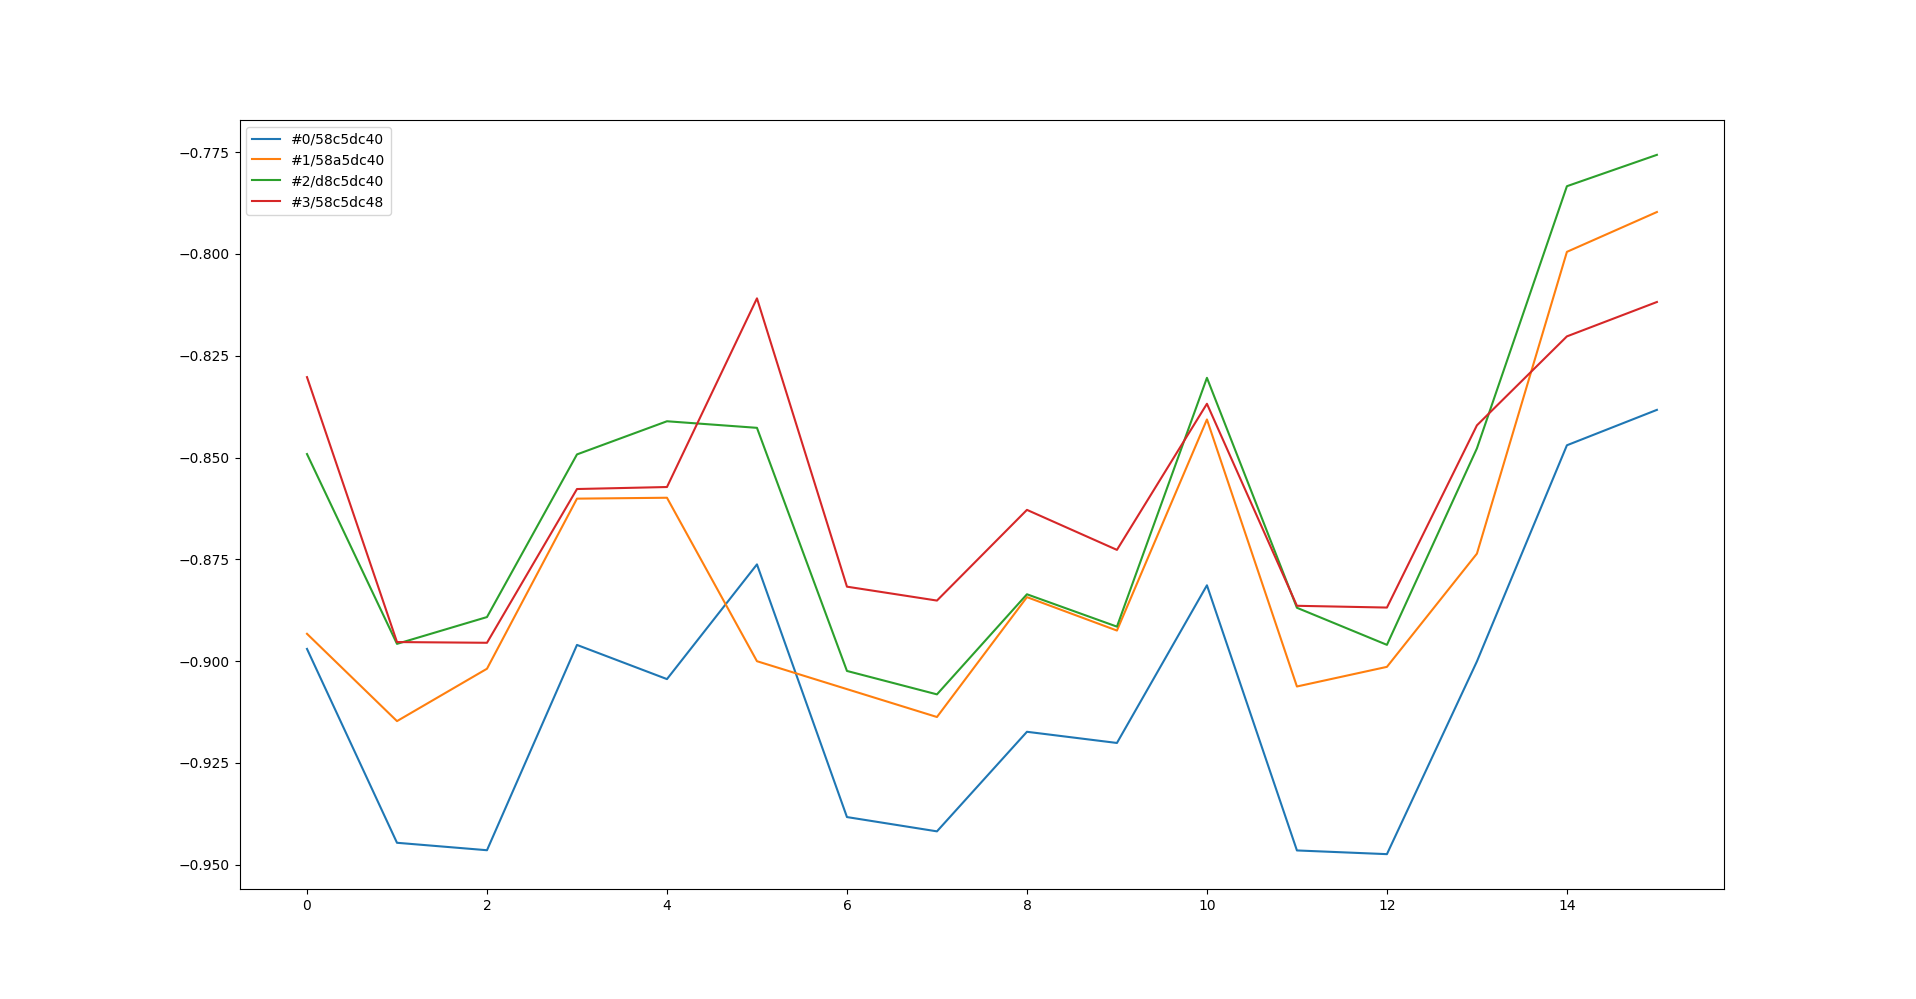
\includegraphics[width=\textwidth]{img/corrs_subkey_word.png}
\end{figure}

Ein Nachteil dieser Verbesserung ist der deutlich erhöhte Aufwand. Da hier pro
32-bit Subkey die Korrelation 15 statt vier Mal berechnet werden muss, ist der
Aufwand etwa um den Faktor $15/4 = 3.75$ größer.

Diese Verbesserung kann mit der Option \verb+-t+ aktiviert werden.




\chapter{Probleme}

\section{Allgemeines}

Bei der Umsetzung des Projekts sind mehrere Probleme aufgetreten. Im Folgenden
wird gezeigt, was einen Angriff erschweren kann und was im Paper
\cite{jungk_bhasin_2017} nicht korrekt ist.


\section{Compiler-Optimierungen}

Sind Optimierungen beim Compiler aktiviert, reduziert sich das Leakage sehr
stark. Mit den Skripten in diesem Projekt war ein Angriff auf eine Variante mit
Compiler-Optimierungen nicht erfolgreich. Bei der Analyse des Assembler-Codes
stellt sich heraus, dass ohne Optimierungen der Zustand dauerhaft vollständig im
RAM liegt und bei jeder Operation die entsprechenden Wert in Register geladen
werden und das Ergebnis anschließend wieder im RAM abgelegt wird. Mit
Optimierungen (gcc -Os) wird pro Runde nur noch wenige Male auf den RAM
zugegriffen, da die Werte für mehrere Operationen in den Registern bleiben.
Außerdem wird die Reihenfolge der Operationen vertauscht. Das hier verwendete
Target (STM32F3) verfügt über einen SRAM-Speicher. Dieser leaked über den
Stromverbrauch Informationen stärker als über die Register sowie als Operand in
den ausgeführten Instruktionen. Dies wird auch im Paper
\cite{adomnicai_fournier_masson_2017} bestätigt.

Ein kommentierter Auszug aus dem Assembler-Code der nicht optimierten Variante
ist in \autoref{lst:asm-not-optimized} bzw. der optimierten Varianten in
\autoref{lst:asm-optimized} zu sehen.

\begin{lstlisting}[caption={Assembler-Code, nicht optimiert (-O0)}, label=lst:asm-not-optimized]
080006cc <chacha_block>:

[...]

 # a += b
 8000704:  68ba        ldr  r2, [r7, #8]
 8000706:  69bb        ldr  r3, [r7, #24]
 8000708:  4413        add  r3, r2
 800070a:  60bb        str  r3, [r7, #8]

 # d ^= a
 800070c:  6bba        ldr  r2, [r7, #56]  ; 0x38
 800070e:  68bb        ldr  r3, [r7, #8]
 8000710:  4053        eors r3, r2
 8000712:  63bb        str  r3, [r7, #56]  ; 0x38

 # d <<= 16 (d >>= 16)
 8000714:  6bbb        ldr  r3, [r7, #56]  ; 0x38
 8000716:  ea4f 4333   mov.w    r3, r3, ror #16
 800071a:  63bb        str  r3, [r7, #56]  ; 0x38

 # c += d
 800071c:  6aba        ldr  r2, [r7, #40]  ; 0x28
 800071e:  6bbb        ldr  r3, [r7, #56]  ; 0x38
 8000720:  4413        add  r3, r2
 8000722:  62bb        str  r3, [r7, #40]  ; 0x28

 # b ^= c
 8000724:  69ba        ldr  r2, [r7, #24]
 8000726:  6abb        ldr  r3, [r7, #40]  ; 0x28
 8000728:  4053        eors r3, r2
 800072a:  61bb        str  r3, [r7, #24]

 # b <<= 12 (b >>= 20)
 800072c:  69bb        ldr  r3, [r7, #24]
 800072e:  ea4f 5333   mov.w    r3, r3, ror #20
 8000732:  61bb        str  r3, [r7, #24]

 # a += b
 8000734:  68ba        ldr  r2, [r7, #8]
 8000736:  69bb        ldr  r3, [r7, #24]
 8000738:  4413        add  r3, r2
 800073a:  60bb        str  r3, [r7, #8]

 # d ^= a
 800073c:  6bba        ldr  r2, [r7, #56]  ; 0x38
 800073e:  68bb        ldr  r3, [r7, #8]
 8000740:  4053        eors r3, r2
 8000742:  63bb        str  r3, [r7, #56]  ; 0x38

[...]
\end{lstlisting}

\begin{lstlisting}[caption={Assembler-Code, optimiert (-Os)}, label=lst:asm-optimized]
0800047c <chacha_block>:

[...]

 # r8: Q0 a
 80004a8:  f8dd 8028   ldr.w  r8, [sp, #40]  ; 0x28

 # r7: Q0 b
 80004ac:  9f0e        ldr  r7, [sp, #56]  ; 0x38

 # r6: Q0 d
 80004ae:  9e16        ldr  r6, [sp, #88]  ; 0x58

 # fp: Q0 c
 80004b0:  f8dd b048   ldr.w  fp, [sp, #72]  ; 0x48

 # ip: Q1 a
 80004b4:  f8dd c02c   ldr.w  ip, [sp, #44]  ; 0x2c

 # r5: Q1 b
 80004b8:  9d0f        ldr  r5, [sp, #60]  ; 0x3c

 # r4: Q1 d
 80004ba:  9c17        ldr  r4, [sp, #92]  ; 0x5c

 # r9: Q1 c
 80004bc:  f8dd 904c   ldr.w  r9, [sp, #76]  ; 0x4c

 # lr: Q2 a
 80004c0:  f8dd e030   ldr.w  lr, [sp, #48]  ; 0x30

 # r1: Q2 b
 80004c4:  9910        ldr  r1, [sp, #64]  ; 0x40

 # r2: Q2 d
 80004c6:  9a18        ldr  r2, [sp, #96]  ; 0x60

 # r0: Q3: a
 80004c8:  980d        ldr  r0, [sp, #52]  ; 0x34

 80004ca:  230a        movs  r3, #10
 80004cc:  9305        str  r3, [sp, #20]


 # Q0: a += b
 80004ce:  44b8        add  r8, r7

 # Q1: a += b
 80004d0:  44ac        add  ip, r5

 # Q0: d ^= a                        # attack subkey #0
 80004d2:  ea88 0606   eor.w  r6, r8, r6

 # Q0: d <<<= 16                     # attack subkey #0
 80004d6:  ea4f 4636   mov.w  r6, r6, ror #16

 # Q1: d ^= a                        # attack subkey #1
 80004da:  ea8c 0404   eor.w  r4, ip, r4

 # Q0: c += d
 80004de:  44b3        add  fp, r6

 # Q1: d <<<= 16                     # attack subkey #1
 80004e0:  ea4f 4434   mov.w  r4, r4, ror #16

 # Q1: c += d
 80004e4:  44a1        add  r9, r4

 # Q0: b ^= c                        # attack subkey #4
 80004e6:  ea8b 0707   eor.w  r7, fp, r7

 # Q0: b <<<= 12                     # attack subkey #4
 80004ea:  ea4f 5737   mov.w  r7, r7, ror #20

 # Q1: b ^= c
 80004ee:  ea89 0505   eor.w  r5, r9, r5

 # Q0: a += b
 80004f2:  44b8        add  r8, r7

 # Q1: b <<<= 12
 80004f4:  ea4f 5535   mov.w  r5, r5, ror #20

 # Q0: d ^= a
 80004f8:  ea86 0608   eor.w  r6, r6, r8

 # Q1: a += b
 80004fc:  44ac        add  ip, r5

 # Q0: r3 = d <<< 8
 80004fe:  ea4f 6336   mov.w  r3, r6, ror #24

 # Q1: d ^= a
 8000502:  ea84 040c   eor.w  r4, r4, ip

 # Q0: c += r3 | c += d
 8000506:  449b        add  fp, r3

 # Q2: a += b
 8000508:  448e        add  lr, r1

 # Q0: sp[6] = r3 | sp[6] = d
 800050a:  9306        str  r3, [sp, #24]

 # Q1: r3 = d <<< 8
 800050c:  ea4f 6334   mov.w  r3, r4, ror #24

 # Q1: c += r3 | c += d
 8000510:  4499        add  r9, r3

 # Q1: sp[7] = r3 | sp[7] = d
 8000512:  9307        str  r3, [sp, #28]

 # Q2: d ^= a
 8000514:  ea8e 0202   eor.w  r2, lr, r2

[...]
\end{lstlisting}



\section{Unklarheiten und Fehler im Paper}

Die genaue Vorgehensweise aus dem Paper \cite{jungk_bhasin_2017} nicht
ersichtlich. Wichtige Informationen fehlen, bei der zweiten Variante mit
eingeschränkter Wahl der Eingabedaten sind mehrere Fehler in der Vorgehensweise.
Mehrere kleinere Tippfehler machen es nicht einfacher.

Laut dem Paper wird die hier getroffene Annahme, dass bei einer symmetrischen
Verteilung immer die negative Korrelation gewählt werden muss, nicht getroffen.
Anstatt dessen sollen beide Möglichkeiten berücksichtigt werden, wobei der
korrekte Kandidat im nächsten Schritt ausgewählt wird, da dort die Korrelation
mit den falschen Subkeys aus dem vorherigen Schritt sehr niedrig ist. Dabei wird
erklärt, dass man bei einer symmetrischen Verteilung beide Fälle berücksichtigt
und beim folgenden Byte (nach dem LSB) $2*256 = 512$ Modelle berechnen muss.
Weiter wird das Vorgehen nicht beschriebenen. Es ist unklar, ob man beim dritten
Byte wieder das gleiche machen muss, wodurch man dann $2*2*256 = 1024$ Modelle
berechnen müsste, sodass man am Ende $2^4 = 16$ 32-bit Subkey-Kandidaten erhält,
oder ob man irgendwie eins der Bytes vorher auswählen muss. Weiter heißt es
nämlich, dass man für das Modell in \autoref{lst:cpa-model-0} immer zwei Subkeys
mit der gleichen absoluten Korrelation erhält. Sofern sich diese Aussage nicht
auf die einzelnen Bytes sondern auf das ganze 32-bit Wort bezieht, würde das
heißen, dass man irgendwie zwischendrin bestimmte Bytes auswählen muss. Dies
wird aber nicht erklärt. Außerdem heißt es, dass man die beiden Subkeys, die man
erhalten hat ausprobieren kann oder den richtigen Subkey mit dem Modell im
\autoref{lst:cpa-model-2} auswählen kann (wie zuvor in diesem Absatz
beschrieben). Auch hier ist unklar, ob sich diese Aussage auf die einzelnen
Bytes oder das ganze 32-bit Wort bezieht. Wenn es sich auf das ganze 32-bit Wort
bezieht, würde das heißen, dass immer noch unklar ist, wie man vorher die
richtigen Bytes auswählen muss. Wenn es sich jedoch auf die Bytes bezieht,
funktioniert die Auswahl nicht richtig, da man aufgrund der Addition im Modell
im \autoref{lst:cpa-model-2} den ganzen 32-bit Subkey aus der ersten Hälfte des
Schlüssels benötigt, am Anfang jedoch nur das erste Byte (LSB) einsetzt.  Durch
das \emph{rotate left} müsste man dann auch im Subkey aus der zweiten Hälfte als
erstes das dritte Byte angreifen, was so nicht im Paper beschrieben ist.

Bei der Erklärung des Ablaufs des Angriffs mit eingeschränkter Möglichkeit die
Eingabe zu steuern sind zwei Fehler enthalten. Erstens soll im
\autoref{itm:calc-v1} des \autoref{sec:attack-2} a2 statt a1 berechnet werden.
Dies kann nicht richtig sein, da dann a2 konstant sein müsste. a2 ist abhängig
von allen Eingabeparametern a0, b0, c0 und d0. Also müssten alle Parameter
konstant sein, womit ein Angriff nicht möglich wäre, da man ansonsten ein Modell
erhalten würde, das für alle Traces den gleichen Stromverbrauch annimmt, was
offensichtlich nicht korrekt ist. Zweitens ist das Modell im letzten Schritt im
Paper nicht korrekt. Da b1 berechnet wird und bis dahin die einzige \emph{rotate
left}-Operation das Wort um 16 Bits rotiert, kann das angegebene Modell mit
einer Rotation um 12 Bits nicht stimmen.

Diese Fehler und Unklarheiten haben die Umsetzung dieses Projekts teils stark
erschwert und lassen Fragen offen, z. B. wie nun die Bytes korrekt ausgewählt
werden, was in diesem Projekt dadurch gelöst wurde, dass nur die Bytes mit einer
negativen Korrelation berücksichtigt werden. Dieser Ansatz basiert jedoch nur
auf Beobachtungen und ist daher möglicherweise nicht korrekt bzw. nicht
allgemeingültig.




\chapter{Auswertung und Bewertung}

Der Angriff hat in den Tests im Rahmen des Projekts bei 500 Traces pro
Aufzeichnung eine Erfolgswahrscheinlichkeit von ca. 99.5\%. Alle
fehlgeschlagenen Aufzeichnungen wurden mit 1000 Traces wiederholt, wobei der
Angriff dann immer erfolgreich verlief. Dies sind gute Ergebnisse, wobei man
berücksichtigen muss, dass diese nur für die nicht optimierte Implementierung
gelten. Der Angriff auf die optimierte Implementierung hat nicht funktioniert.
Anhand der Analyse mit spezifischem TVLA bzw. NICV ist zu sehen, dass Leakage
vorhanden ist, aber stark reduziert. Mit erhöhtem Aufwand wäre hier ein Angriff
also vermutlich auch möglich. Zu diesem Schluss kamen auch die Autoren des
Papers \cite{jungk_bhasin_2017}.

Sollte ein Angriff auf die optimierte Implementierung erfolgreich sein, hat dies
eine nicht unbeachtliche Relevanz, da die getroffenen Annahmen realistisch sind.
Es werden weder der Klar- noch der Schlüsseltext benötigt. Lediglich der Counter
und das erste Wort der Nonce muss konstant und bekannt, sowie die Möglichkeit,
die letzten beiden Wörter der Nonce steuern zu können, muss gegeben sein. Wie
die Autoren des Papers \cite{jungk_bhasin_2017} es beschreiben, sind dies
Annahmen, die getroffen werden können, da beim Message Authentication Code
Poly1305 der Counter auf 0 fixiert ist und die Nonce bekannt ist.

Da ChaCha eine von drei möglichen Chiffren im TLSv1.3-Standard ist, wird ChaCha
vermutlich auch in Zukunft verbreitet benutzt, weshalb ein erfolgreicher Angriff
eine Gefährdung für viele Geräte darstellt.




\chapter{Weitere Anwendungen}

In diesem Projekt sind neben den bereits vorgestellten Anwendungen Weitere
enthalten.

\begin{description}
    \item[attack\_test.py] Mit diesem Skript kann man testen, wie gut der
        Angriff funktioniert, indem der Angriff gleichzeitig auf mehrere Traces
        ausgeführt und am Ende eine Statistik der Erfolge bzw. Misserfolge
        angezeigt wird.

    \item[test\_chacha\_implementation.py] Mit diesem Skript kann die ChaCha
        Implementierung auf dem Target sowie die korrekte Kommunikation mit
        einem Known-Answer-Test getestet werden.
\end{description}

Alle Anwendungen haben möglicherweise weitere Parameter, die hier nicht erwähnt
wurden. Diese sind im Programm selbst dokumentiert und lassen sich immer mit der
Option \verb+-h+ anzeigen.




\printbibliography




\end{document}

